\chapter{Dizajn i implementacija}

Proces dizajniranja i implementacije, odnosno, projektovanja sistema, može se posmatrati kao proces rješavanja problema. Sam proces zahtijeva da se prvo pronađe niz mogućih rješenja, a zatim od pronađenih izabere najbolje rješenje. Svaki sistem mora biti projektovan na vrijeme, u okviru sredstava, imati prihvatljive performanse, te biti ispravan i pouzdan. Dobro projektovan sistem ne treba samo zadovoljiti trenutne zahtjeve, već i imati mogućnost da se prilagodi novim zahtjevima. 

Neki veliki lunapark obično projektuje tim ljudi. Određen broj ljudi zadužen je za planiranje arhitekture lunaparka, drugi tim ljudi zadužen je za planiranje tehničkog dijela, a posebni timovi zaduženi su za sam proces gradnje, a često sistem ima i tim zadužen za marketing. S obzirom da je ovo studentski projekt, simulacija lunaparka, sav posao, umjesto timova, radi jedan student. Sistem je sastavljen od podsistema, koje čine određene komponente uklopljene u objekte, najčešće napravljene od kartona. Sve to povezuje Arduino Mega mikrokontroler, programiran kôdom predstavljenim u nastavku seminarskog rada. 

 
\section{Maketa sistema}
Sistem se sastoji od jako detaljne makete, te elektronskih komponenti koje mu daju funkcionalnost. Dijelovi sistema su karusel, vrtuljak, šoljice, vračara, te igra koja uključuje sortiranje boja. Svi dijelovi su raspoređeni u ručno napravljene šatore ili na postolja. 
 \begin{figure}[h!]
  \centering
  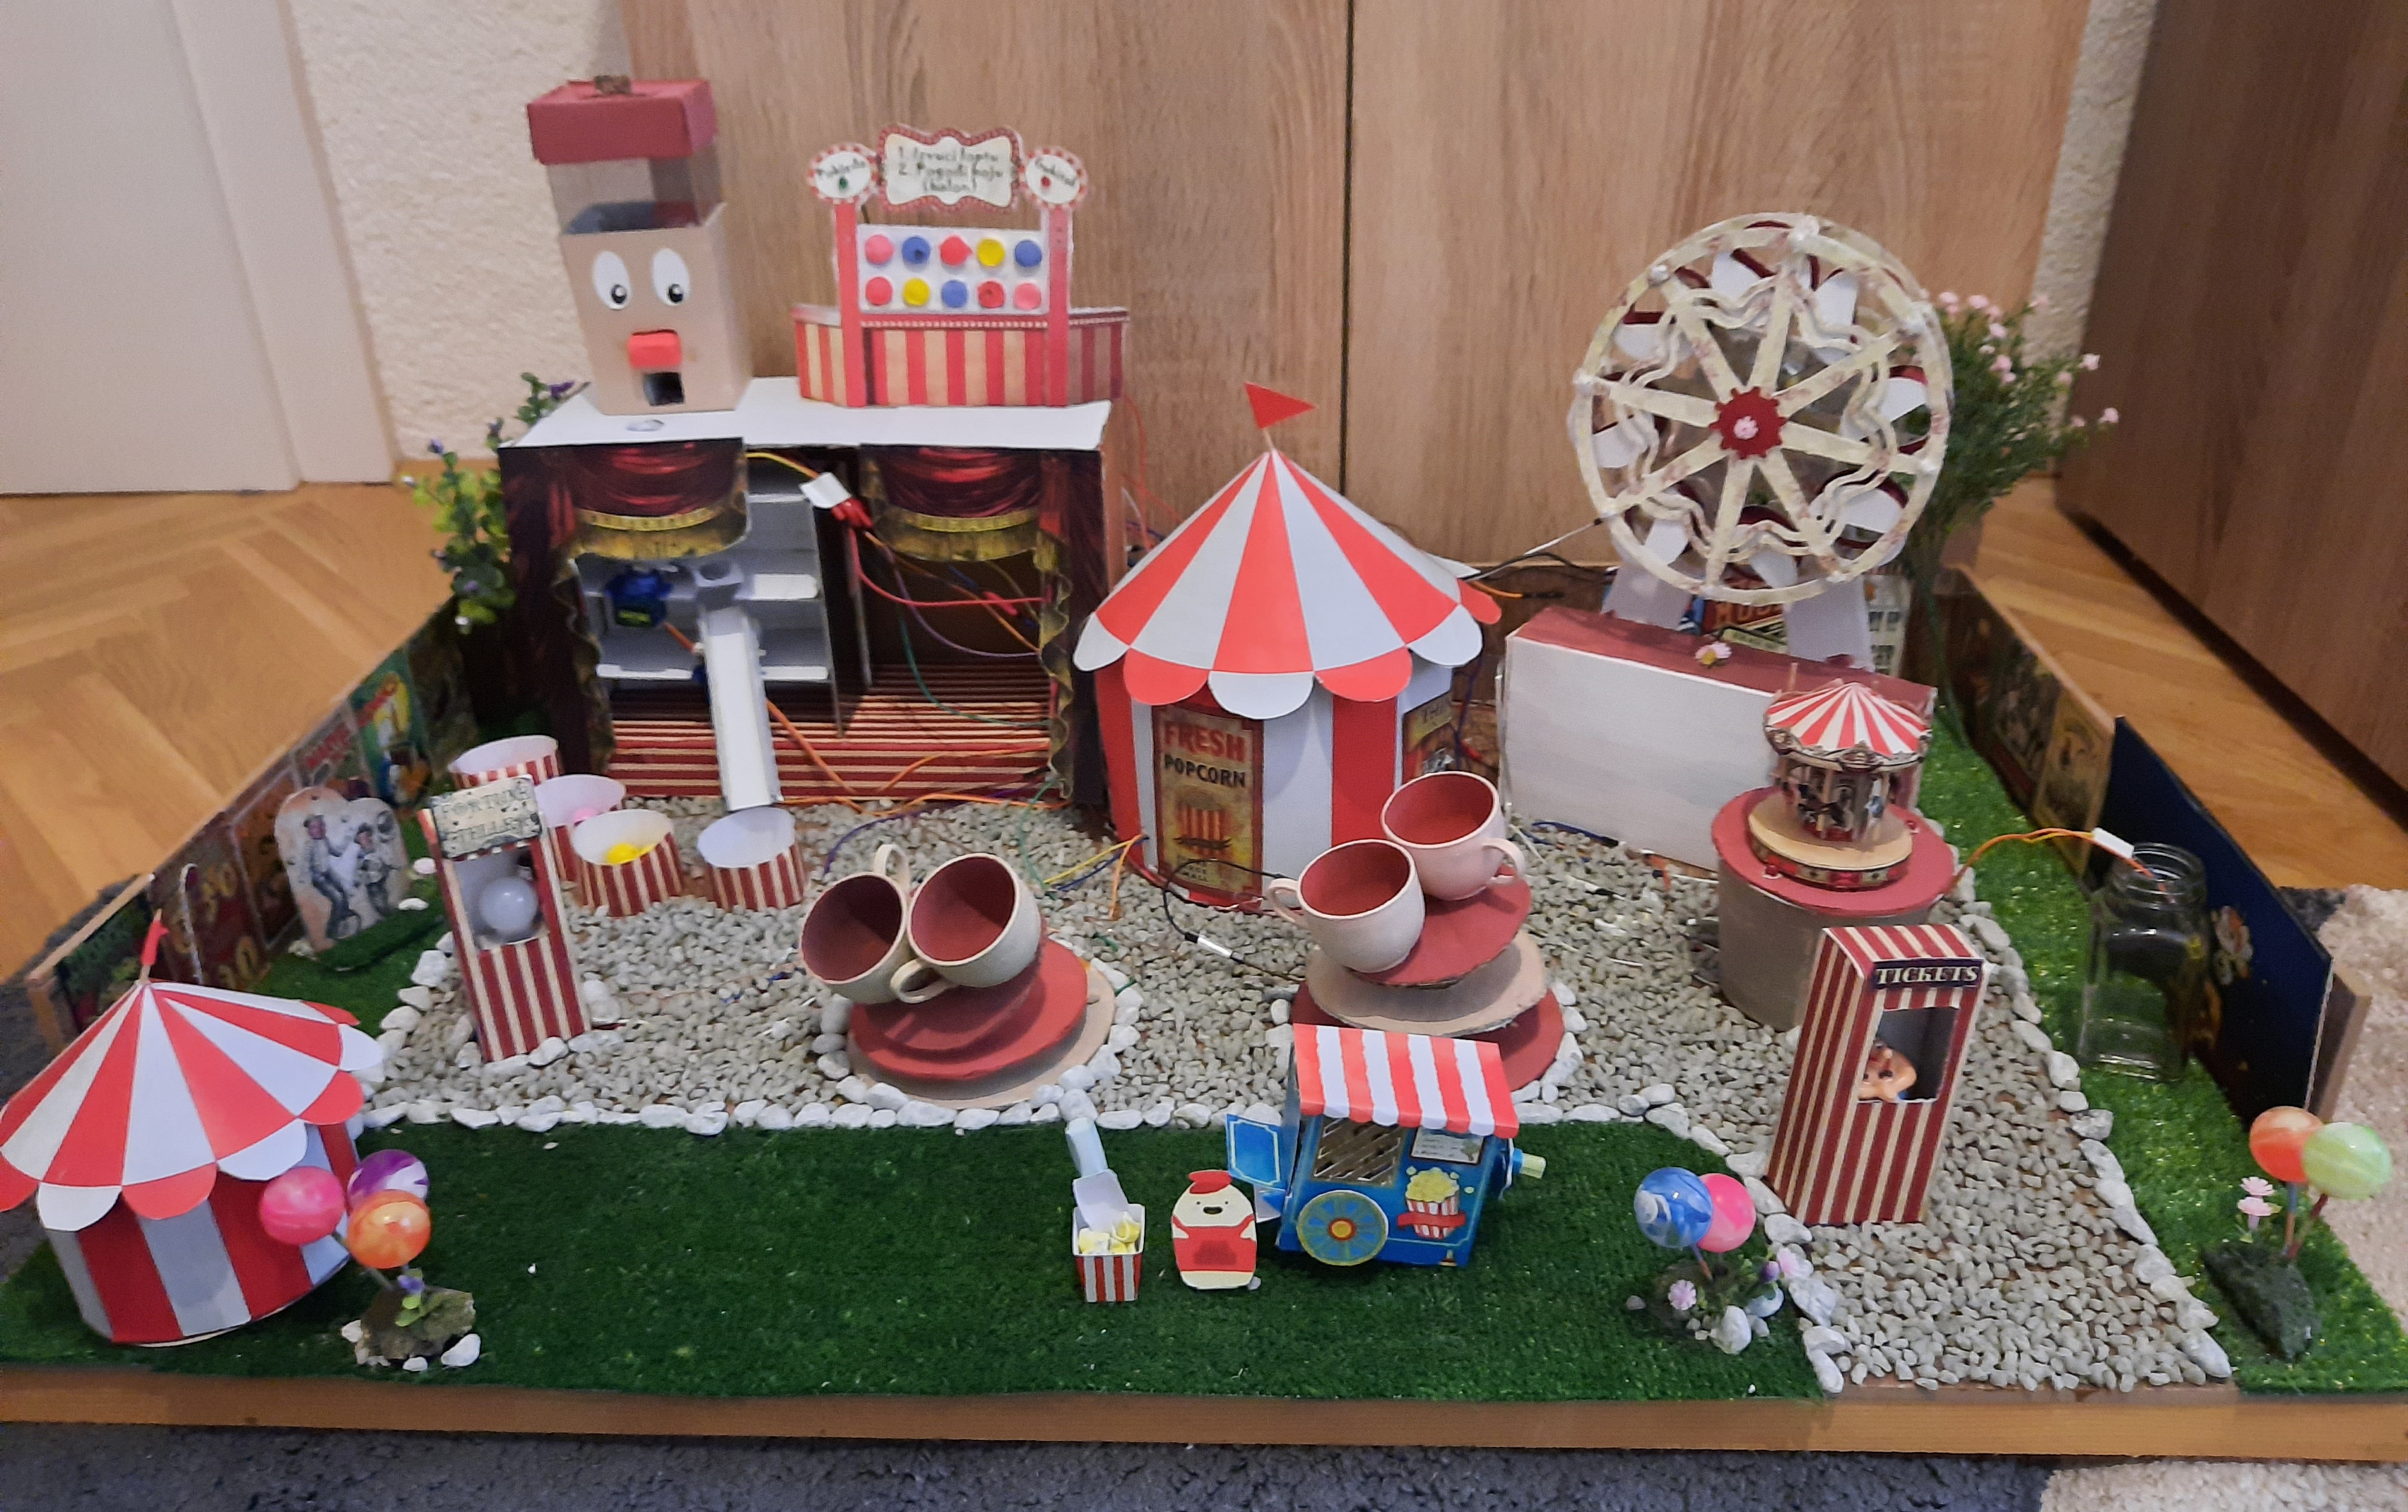
\includegraphics[width=0.7\textwidth]{maketa3}
  \caption{Maketa sistema}
  \label{fig:Slika_Maketa}
\end{figure}

Maketa sistema prikazana je na slici \ref{fig:Slika_Maketa}. Podloga je napravljena od šperploče, s tim da su zidovi, radi sigurnosti i stabilnosti, učvršćeni letvicama. Za nju nije korišteno ljepilo, već je pričvršćena ekserima. Posteri na zidovima su isprintani. Većina dijelova je napravljena od kartona, na koji su zalijepljeni šabloni od papira, koji su ili napravljeni u Photoshopu, ili preuzeti s Interneta, ali prilagođeni projektu. 

Shema sistema prikazana je na slici \ref{fig:Slika_shema}.
\begin{figure}[h!]
  \centering
  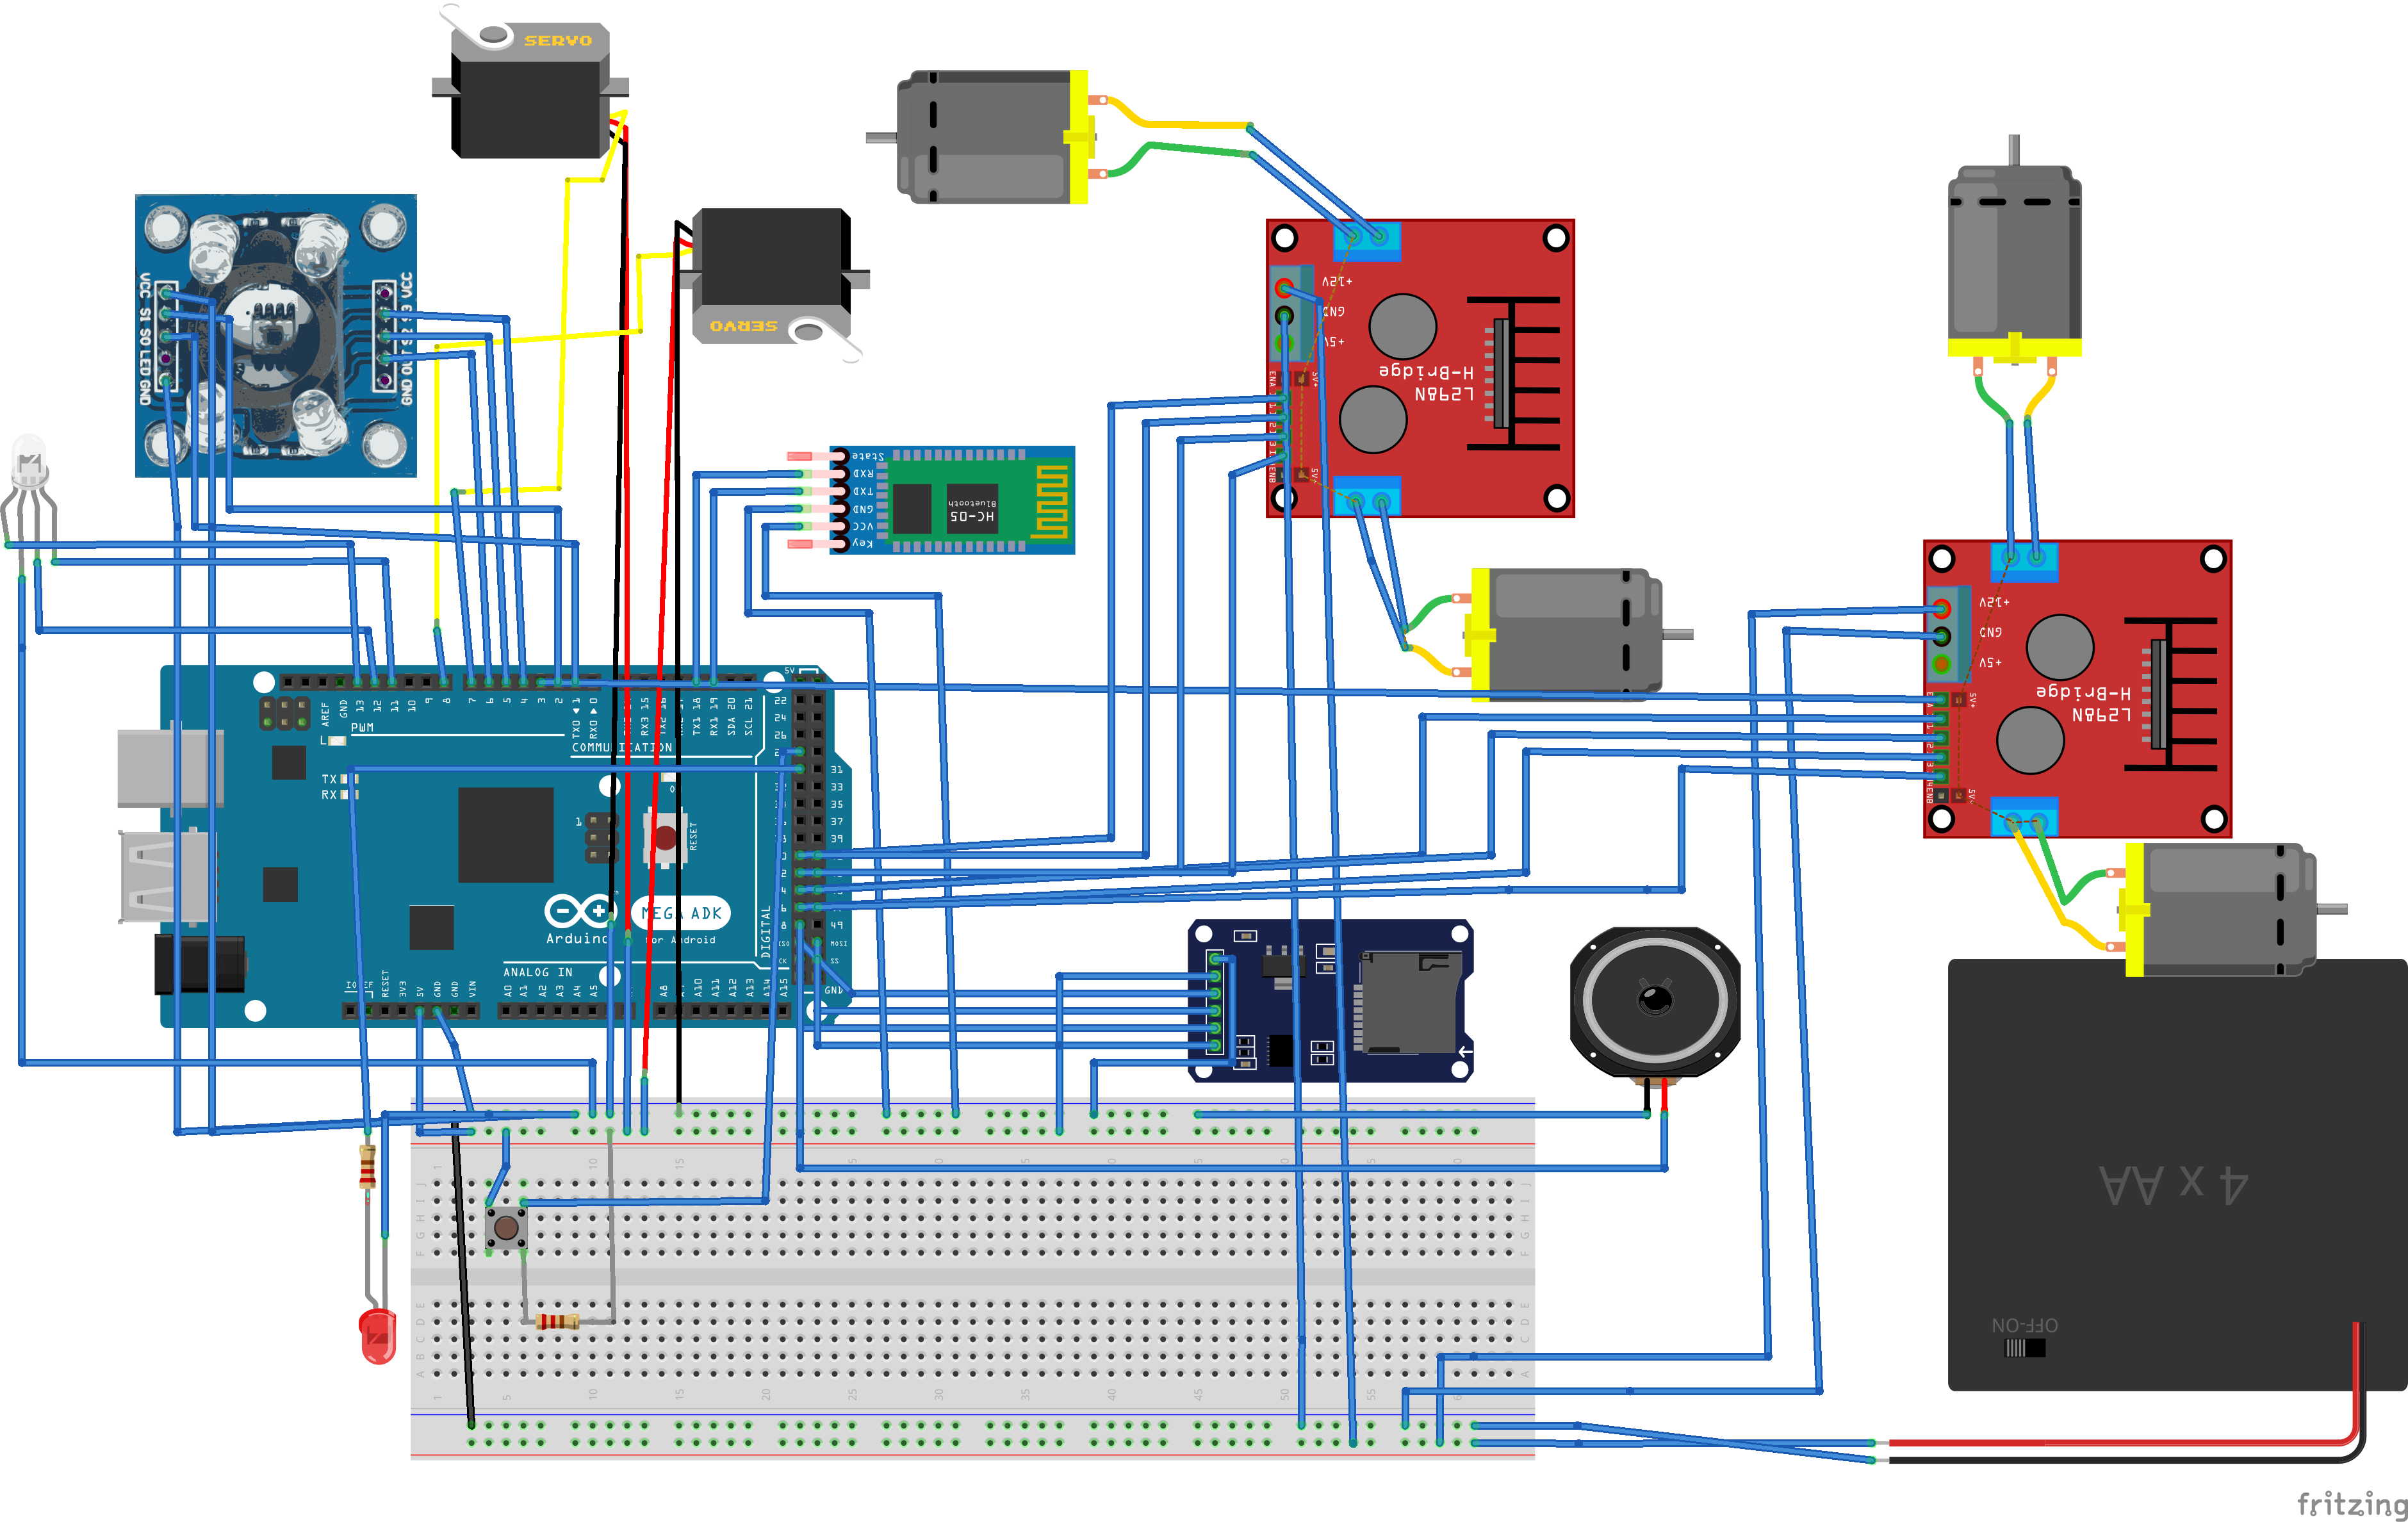
\includegraphics[width=0.7\textwidth]{shema2}
  \caption{Shema sistema}
  \label{fig:Slika_shema}
\end{figure}

Shema je malo pojednostavljena, duple diode i push buttoni nisu stavljeni. Električna shema prikazana je na slici \ref{fig:Slika_elshema}. 

\begin{figure}[h!]
  \centering
  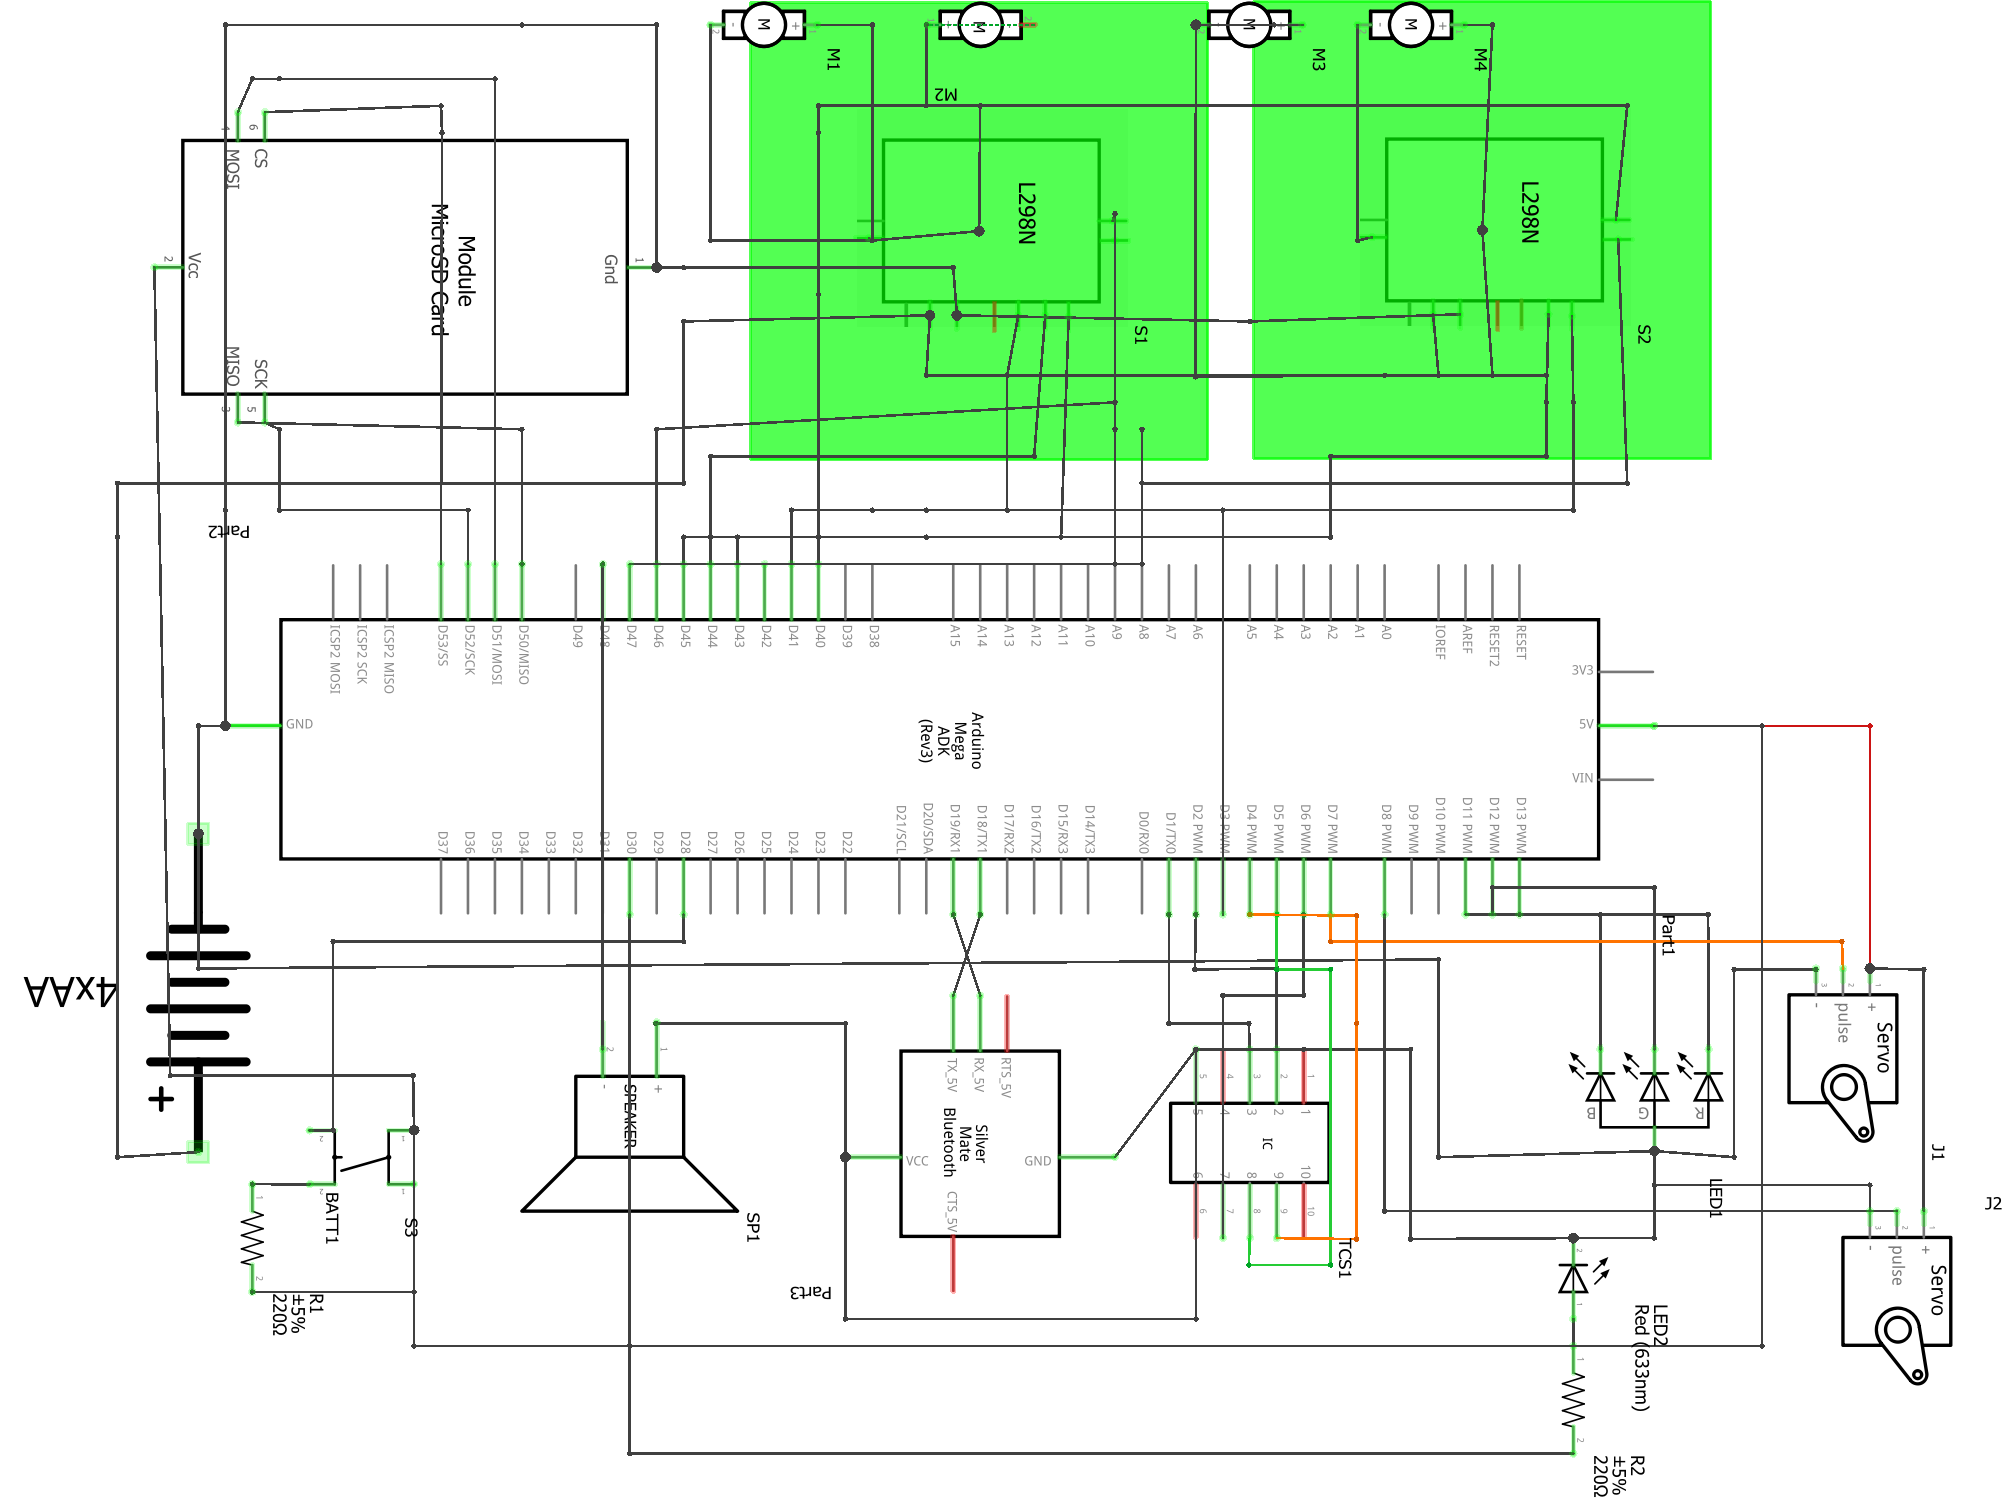
\includegraphics[width=0.7\textwidth]{elshema}
  \caption{Električna shema sistema}
  \label{fig:Slika_elshema}
\end{figure}

Na slici \ref{fig:Slika_dijagram} prikazan je blokovski dijagram sistema. Na dijagramu su označeni ulazi i izlazi iz sistema. Ulazi u sistem su napajanje, poruke primljene putem bluetootha, te informacije od senzora, modula i push buttona. Izlazi su signali koji se daju LED diodama, servo motorima, zvučniku, te motor driverima, koji ih prosljeđuju DC motorima. Motor driveri, osim signala od mikrokontrolera, primaju i vlastito napajanje, pošto nije dobro DC motore napajati zajedno s mikrokontrolerom. 

\begin{figure}[h!]
  \centering
  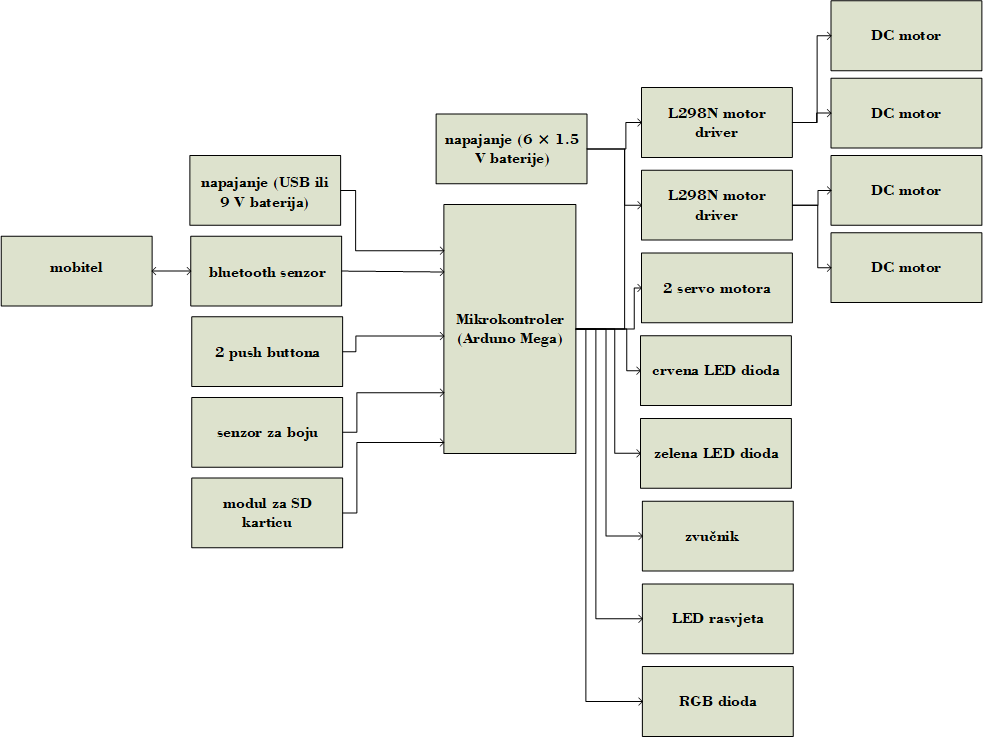
\includegraphics[width=0.7\textwidth]{dijagram}
  \caption{Blokovski dijagram sistema}
  \label{fig:Slika_dijagram}
\end{figure}

Osim komponenti, sistem se sastoji od Android aplikacije. Aplikacijom se simulira sistem za ulaznice u sistem. Korisnik pokaže ulaznicu radniku koji ima aplikaciju na mobitelu, te ako je ona odgovarajuća, korisnik može ući u sistem. Kad se pokrene Android aplikacija, otvori se prozor za prikazivanje ulaznice, kao na slici \ref{fig:Slika_prikazi}.

\begin{figure}[h!]
  \centering
  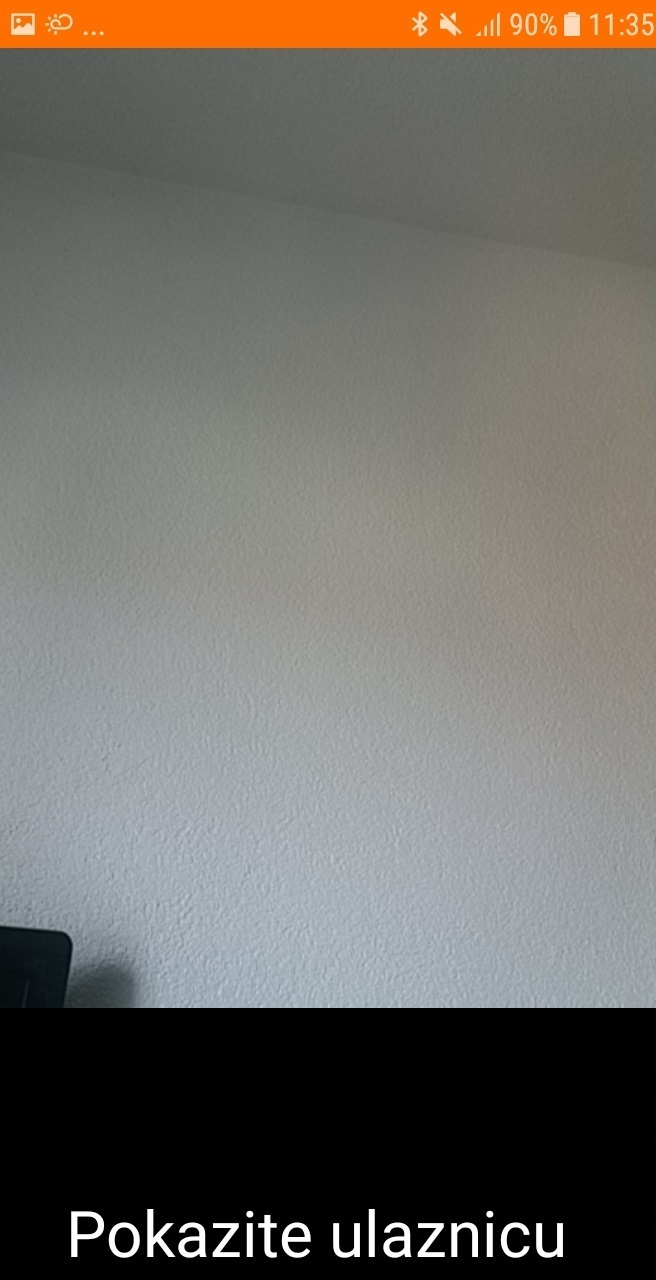
\includegraphics[width=0.25\textwidth]{prikazi}
  \caption{Izbornik za prikazivanje ulaznice}
  \label{fig:Slika_prikazi}
\end{figure}

Izrađene ulaznice prikazane su na slici \ref{fig:Slika_Ulaznice}. 
\newpage
\begin{figure}[h!]
  \centering
  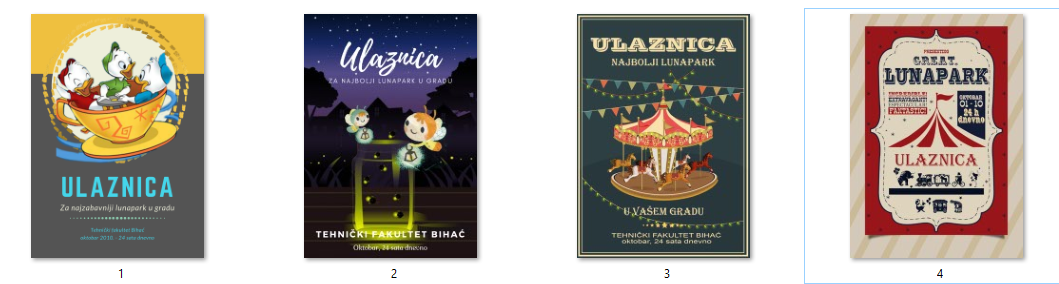
\includegraphics[width=0.7\textwidth]{ulaznice.png}
  \caption{Ulaznice za sistem}
  \label{fig:Slika_Ulaznice}
\end{figure}

Kad aplikacija prepozna ulaznicu, pokaže se izbornik za pretragu i povezivanje, kao na slici \ref{fig:Slika_izbornik}. Na istoj slici je prikazana i lista bluetooth uređaja koja se prikaže kad se pritisne izbornik za pretragu. Nakon povezivanja, otvori se izbornik kao na slici \ref{fig:Slika_kraj}. Uz pomoć ovog izbornika, korisnik upravlja sistemom.  
\begin{figure}[h!]
  \centering
  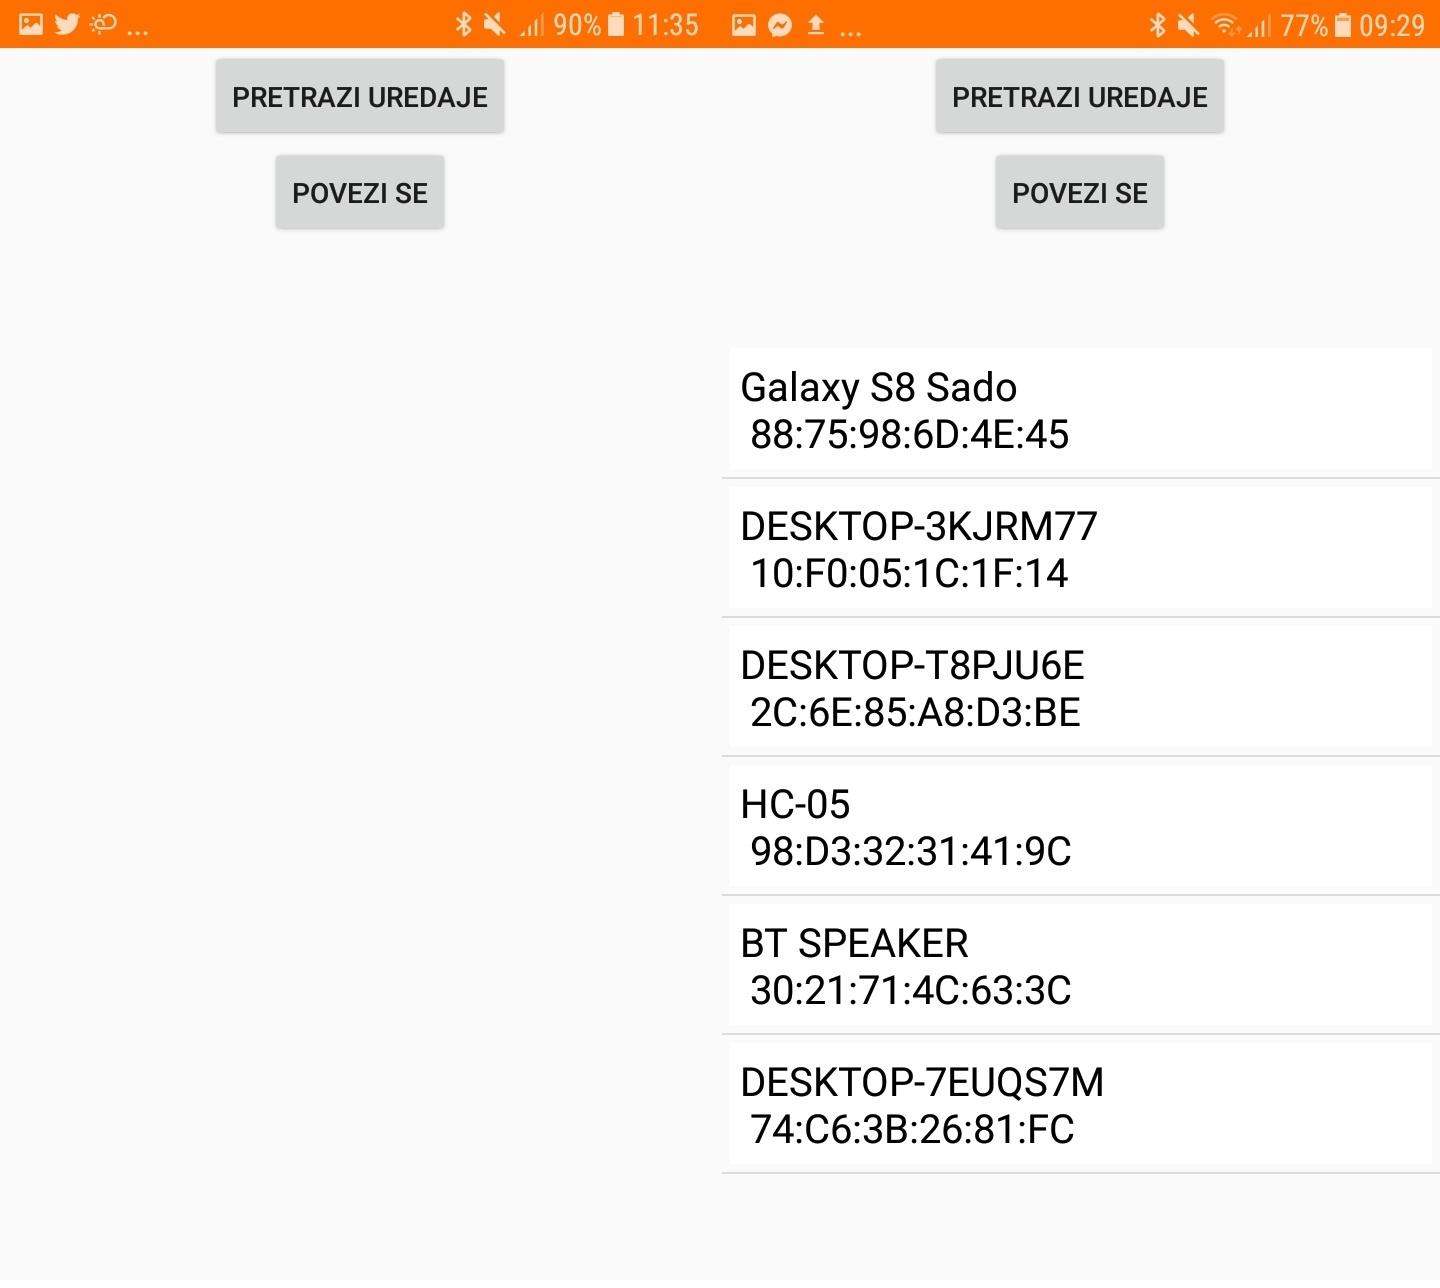
\includegraphics[width=0.5\textwidth]{pretrazibt}
  \caption{Izbornik za pretragu i povezivanje}
  \label{fig:Slika_izbornik}
\end{figure}

Blokovski dijagram podsistema za ulaznice prikazan je na slici \ref{fig:Slika_dijagram2}. Akvizicija ulaznice vrši se uz pomoć kamere mobitela. Prepoznavanje ulaznica vrši se uz pomoć neuronske mreže, koja šalje informaciju o prepoznavanju mobilnoj aplikaciji. Aplikacija potom komunicira sa sistemom uz pomoć bluetooth modula.

\begin{figure}[h!]
  \centering
  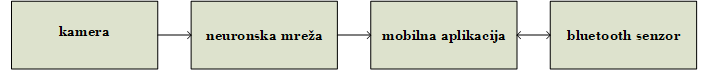
\includegraphics[width=0.7\textwidth]{dijagram2}
  \caption{Blokovski dijagram sistema za ulaznice}
  \label{fig:Slika_dijagram2}
\end{figure}

Komponente koje su iskorištene za kreiranje lunaparka su: Arduino Mega 2560 pločica, 4 različita DC motora (2 obična DC motora od 3 V, jedan od 12 V, a jedan sa zupčanicima), L298N driver za motore, modul za SD karticu, zvučnik, HC-05 Bluetooth modul, RGB dioda, senzor za boju, 2 servo motora, 3 push buttona, eskperimentalna pločica, te diode i otpornici.

\begin{figure}[h!]
  \centering
  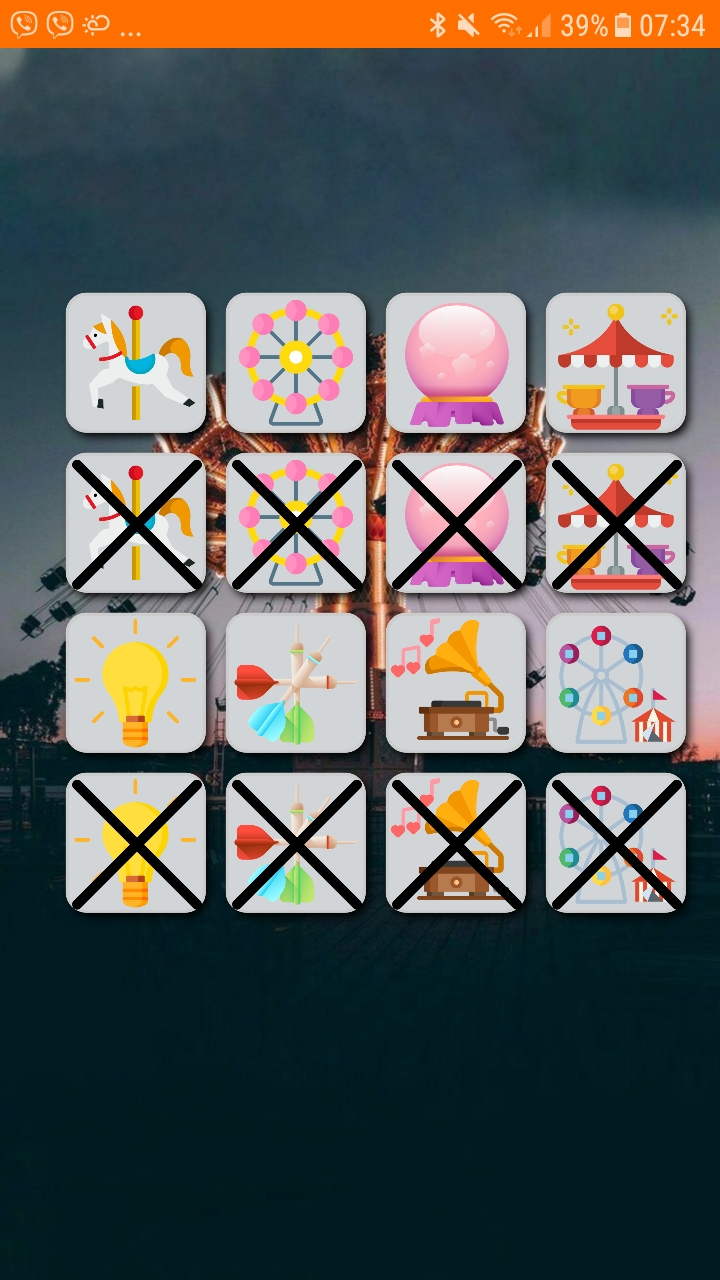
\includegraphics[width=0.25\textwidth]{kraj2}
  \caption{Finalni izbornik aplikacije}
  \label{fig:Slika_kraj}
\end{figure}

Većina komponenti smještena je u veliki šator na sredini makete, kako ne bi kvarile sam dizajn projekta. Unutrašnjost šatora prikazana je na slici \ref{fig:Slika_sator}. Posebna pažnja morala je da se obrati na to da komponente budu povezane s odgovarajućim pinovima. Bluetooth modul morao je biti povezan sa serijskim portom, kojih Arduino Mega ima čak 4, modul za SD karticu morao je biti povezan sa posljednja 4 pina, pošto su to MISO (\textit{Master In Slave Out}), MOSI (\textit{Master Out Slave In}), SCK (\textit{Serial Clock}) i SS (\textit{Slave Select}) pinovi, pinovi namijenjeni za asihnhronu komunikaciju u kojoj je Arduino pločica master element, dok su RGB dioda i kontrola brzine motora morali biti povezani sa PWM pinovima.
\begin{figure}[h!]
  \centering
  \includegraphics[width=0.5\textwidth]{unutrasnjost}
  \caption{Unutrašnjost šatora u kojem je skrivena većina komponenti}
  \label{fig:Slika_sator}
\end{figure}

Motorima u sistemu obezbijeđeno je vlastito napajanje, pomoću paketa od 6 AA baterija od 1,5 V, dok se Arduino pločica i ostale komponente mogu napajati uz pomoć USB-a, odnosno, električne energije, ili baterije od 9 V. Na ovaj način sistem je osiguran od pregaranja, a istovremeno je omogućeno dovoljno energije da se veliki broj motora kreće kako je planirano.
\